\chapter{Context of the work}
\minitoc
\newpage

\setcounter{secnumdepth}{0} % Set the section counter to 0 so next section is not counted in toc
% ----------------------- Introduction ----------------------- %
\section{Introduction}
This chapter introduces the general context of this report.
We start by presenting the frame of the project as well as the host company.
Then comes the enumeration of the problems which led to the realization of the project.
We wrap it up by defining the methodology we’ve followed to carry out our work.

\setcounter{secnumdepth}{2} % Resume counting the sections for the toc with a depth of 2 (Sections and sub-sections)
% ----------------------- General framework of the internship ----------------------- %
\section{General framework of the internship}
This project was carried out within the frame of obtaining a bachelor’s degree in Computer Science at the Higher Institute of Informatics and Mathematics of Monastir (ISIMM).
The internship took place fully remotely at Incedo Services GmbH for five months starting from the 15th of January 2024 to the 15th of June 2024 with the purpose of further developing an existing software solution of the company as well as working on a new feature, which is the reward system.

% ----------------------- Company overview ----------------------- %
\section{Company overview}
This section introduces the host company {\bf Incedo Services GmbH} as well as the services it offers.
\subsection{About Incedo}
"We are a young software development and consulting firm located in Stuttgart.
We help our clients to develop exciting digital products and solutions and we also love to bring our own ideas into life from time to time." \cite{about-incedo}
\begin{figure}[H]
    \centering
    \makebox[\textwidth]{
\includegraphics[width=12cm]{src/assets/images/incedo-logo_bg-trans-white_rgb.png}}
    \caption{Logo of Incedo Services GmbH}
    \label{fig:logo-of-incedo}
\end{figure}

\subsection{Incedo's services}
\subsubsection*{\underline{Consulting}}
Incedo helps its clients overcome two main challenges:
\begin{itemize}
    \item Develop a product that somebody actually needs and that creates enough value to form a profitable business case.
    \item Ensuring that (large) IT-projects are finished in time \& budget with a result that satisfies the actual users/clients of the developed software solution.
\end{itemize}

\subsubsection*{\underline{Development}}
Incedo develops software for clients, as well as for the company itself.
\begin{figure}[H]
    \centering
    \makebox[\textwidth]{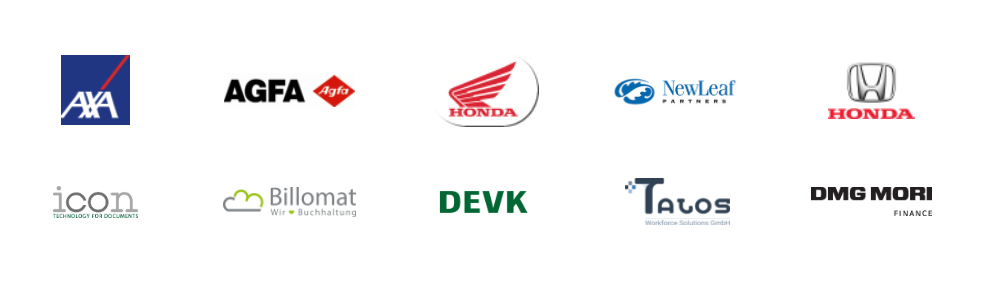
\includegraphics[width=\linewidth]{src/assets/images/selection-of-clients.JPG}}
    \caption{Selection of Incedo clients}
    \label{fig:selection-of-incedo-clients}
\end{figure}

% ----------------------- Stating the problem ----------------------- %
\section{About Aermax}

Aermax is a company founded by our client, Max Wörner, based in Stuttgart, Germany. Aermax specializes in industrial climbing services, providing skilled professionals for high-altitude or deep-location tasks using rope access techniques. An industrial climber is a trained specialist whose work area is usually at great heights or depths. During operations, industrial climbers use a method called rope access technique. This method allows craftsmen to perform their work in hard-to-reach places without the need for scaffolding or lifts.

\subsection*{Key Advantages of Industrial Climbers}
\begin{itemize}
  \item Ability to work at any height or depth
  \item Flexible deployment using ropes
  \item Performing tasks without scaffolding or lifts
  \item Cost-effective and efficient
  \item Operation without disrupting business or production processes
  \item Short preparation time
  \item Capability for short-notice emergency deployments
\end{itemize}

By leveraging these advantages, Aermax ensures that their services are not only effective but also adaptable to various challenging environments, maintaining high standards of safety and efficiency.

\begin{figure}[H]
    \centering
    \makebox[\textwidth]{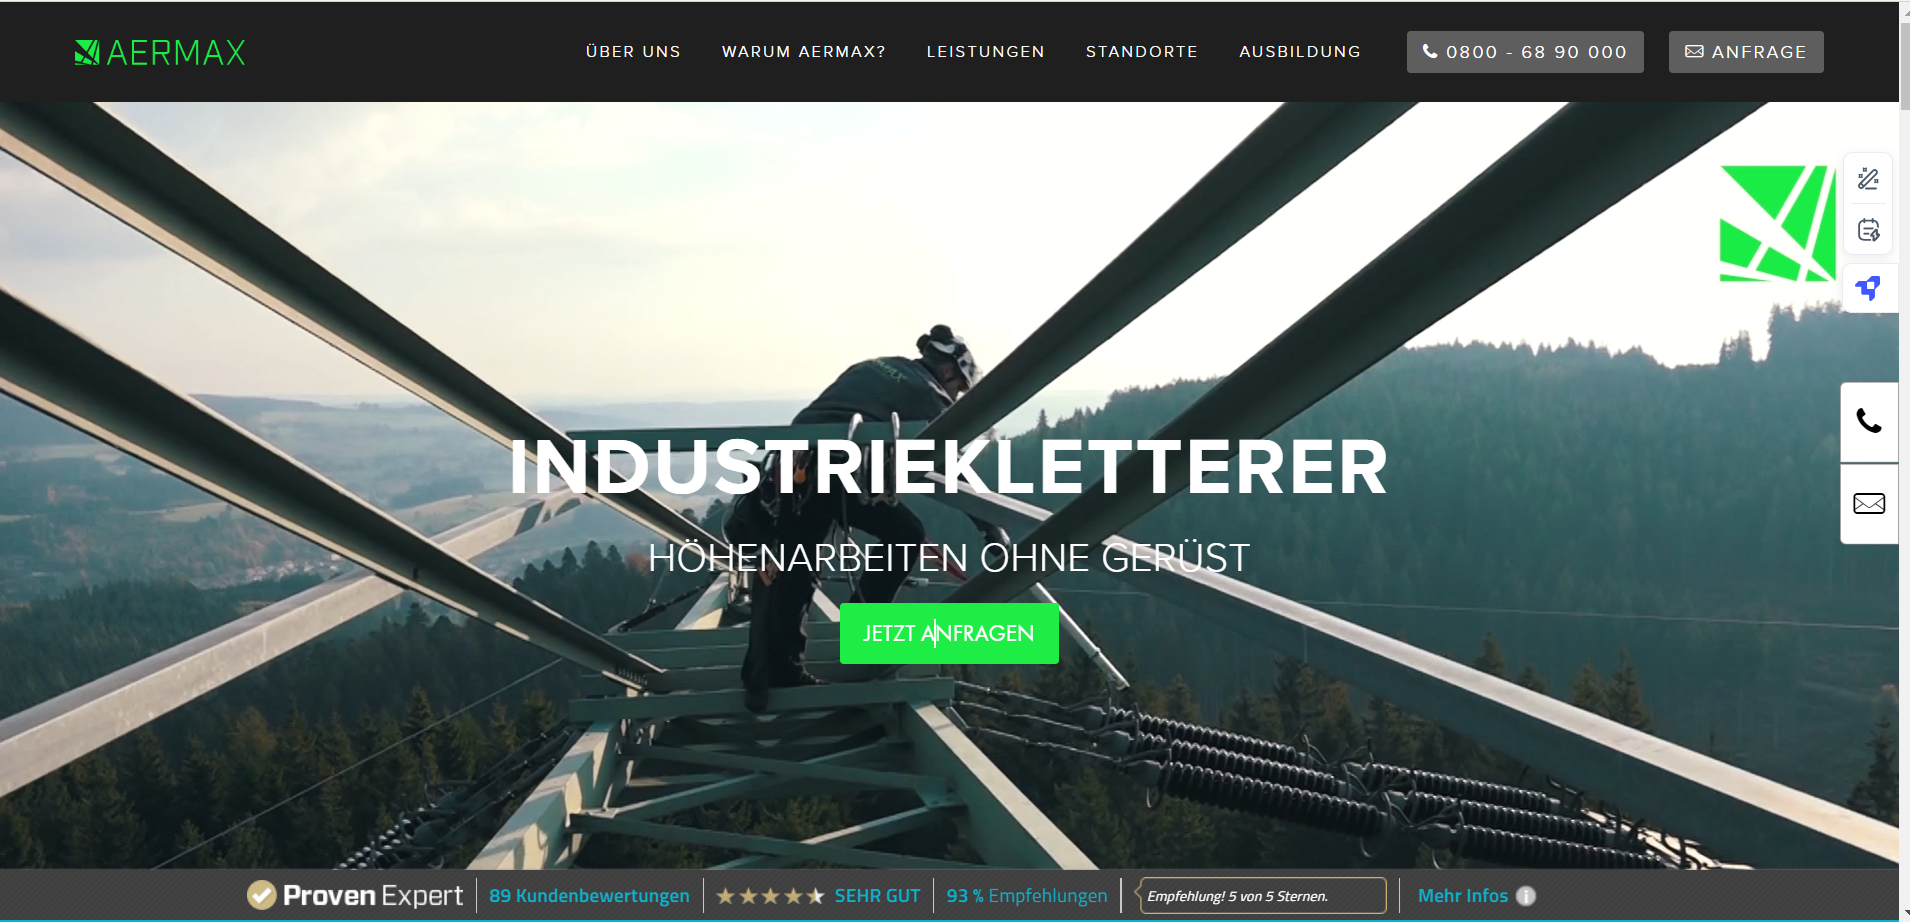
\includegraphics[width=12cm]{src/assets/images/aermax.PNG}}
    \caption{Aermax’s website}
    \label{fig:aermax-website}
\end{figure}

The client wanted to develop a platform to manage all their work, especially between employees (interns) and subcontractors (externs).

\section{Competitor Benchmarking}
In this section, we’ll analyze the Aermax platform, reviewing its features, capabilities, and performance. Our goal is to identify its strengths and areas for improvement, comparing it with industry standards. This evaluation will guide the enhancement of our platform, ensuring it meets the unique demands of high-altitude project management efficiently.

\subsection{Competitors Selection}
In our investigation of existing solutions, we meticulously assessed various platforms and pinpointed four that most closely meet our specific requirements. We will provide a summary of these selected solutions, emphasizing their main features and functionalities.

\subsection{Blauarbeit}
Blauarbeit is an online platform where German citizens can look for experts to help with hard and sometimes dangerous tasks like structure and fixing effects in their homes or workplaces. It's like a big directory filled with experts who are good at fixing effects like broken pipes, electrical problems, or erecting new structures. This makes it easy for anyone to find the right person for the job without having to search all over the place. Plus, Blauarbeit makes sure that all the workers are dependable and secure, so people can feel confident about hiring them. Whether it's repairing a dense roof or cleaning at a high altitude and dangerous place.

\begin{figure}[H]
    \centering
    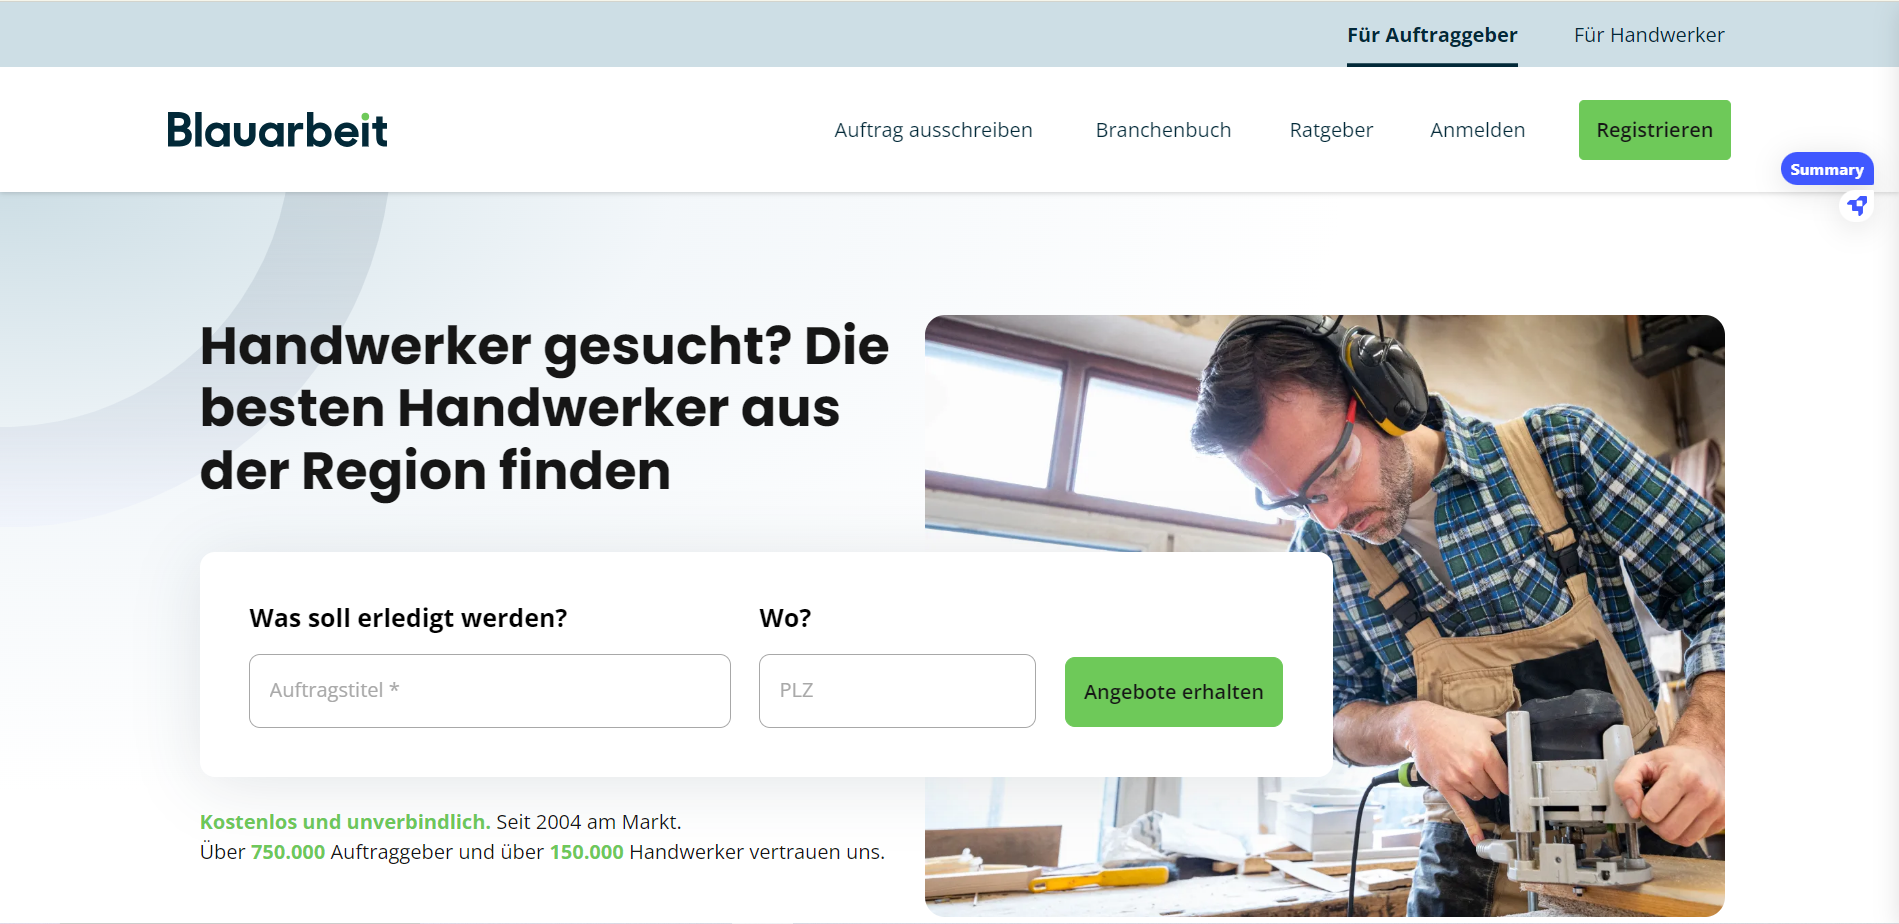
\includegraphics[width=\linewidth]{src/assets/chapters/Blaurabeit.PNG}
    \caption{Blaurabeit Homepage}
    \label{fig:blaurabeit_image}
\end{figure}

\subsection{IRATA Hub}
IRATA Hub is a specialized digital platform catering to the unique needs of companies and technicians engaged in industrial rope access projects. Offering a range of functionalities, it simplifies project management while ensuring adherence to industry standards. From managing certification records and tracking training courses to scheduling equipment inspections and centralizing project documentation, IRATA Hub streamlines administrative tasks with efficiency. Moreover, it promotes safety by providing technicians with up-to-date safety procedures and facilitating real-time communication among project teams. With its comprehensive features, IRATA Hub serves as a valuable tool for enhancing project management and safety in industrial rope access projects.

\begin{figure}[H]
    \centering
    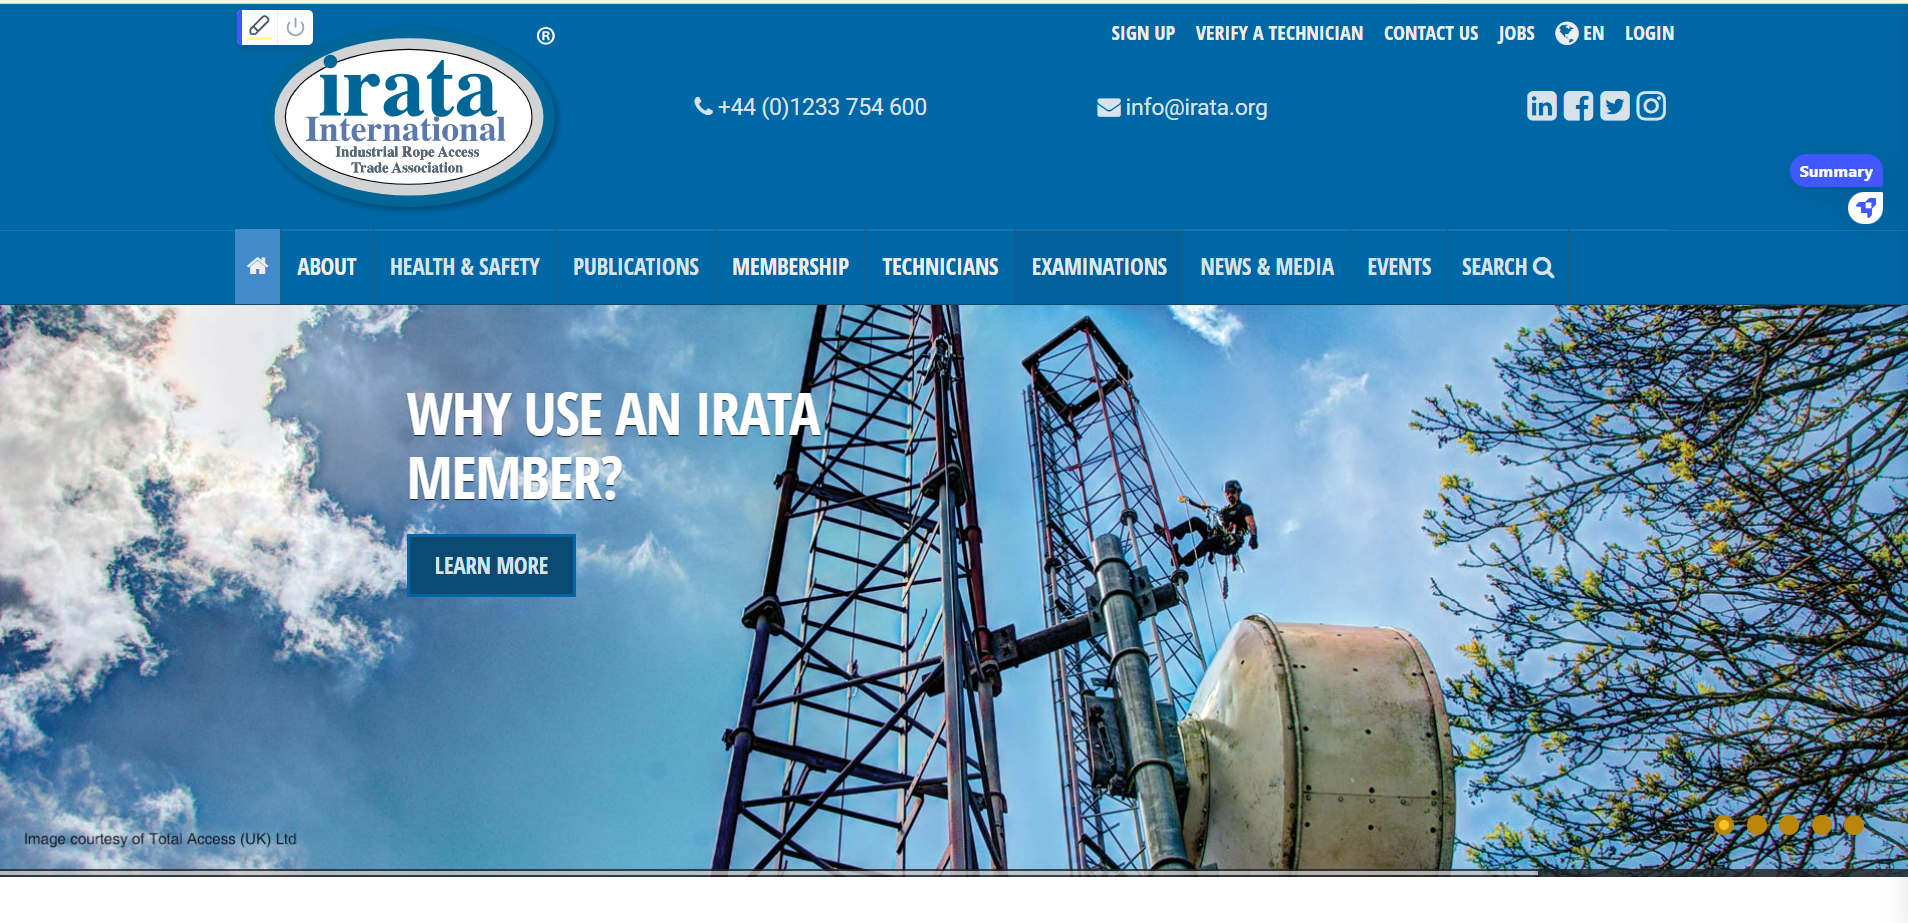
\includegraphics[width=\linewidth]{src/assets/chapters/iratahub.PNG}
    \caption{IRATAHUB Homepage}
    \label{fig:iratahub_image}
\end{figure}

\subsection{Fieldwire}
Fieldwire is a robust project management software designed for construction teams to streamline collaboration and task management. Its key functionalities include task management, plan viewing, issue tracking, and real-time communication. With Fieldwire, users can create and assign tasks, upload and view construction plans, document issues and observations, and communicate with team members instantly. The platform facilitates seamless coordination among team members, allowing for efficient project planning and execution. By centralizing project information and communication, Fieldwire helps construction teams stay organized, ensure project accuracy, and meet project deadlines effectively.

\begin{figure}[H]
    \centering
    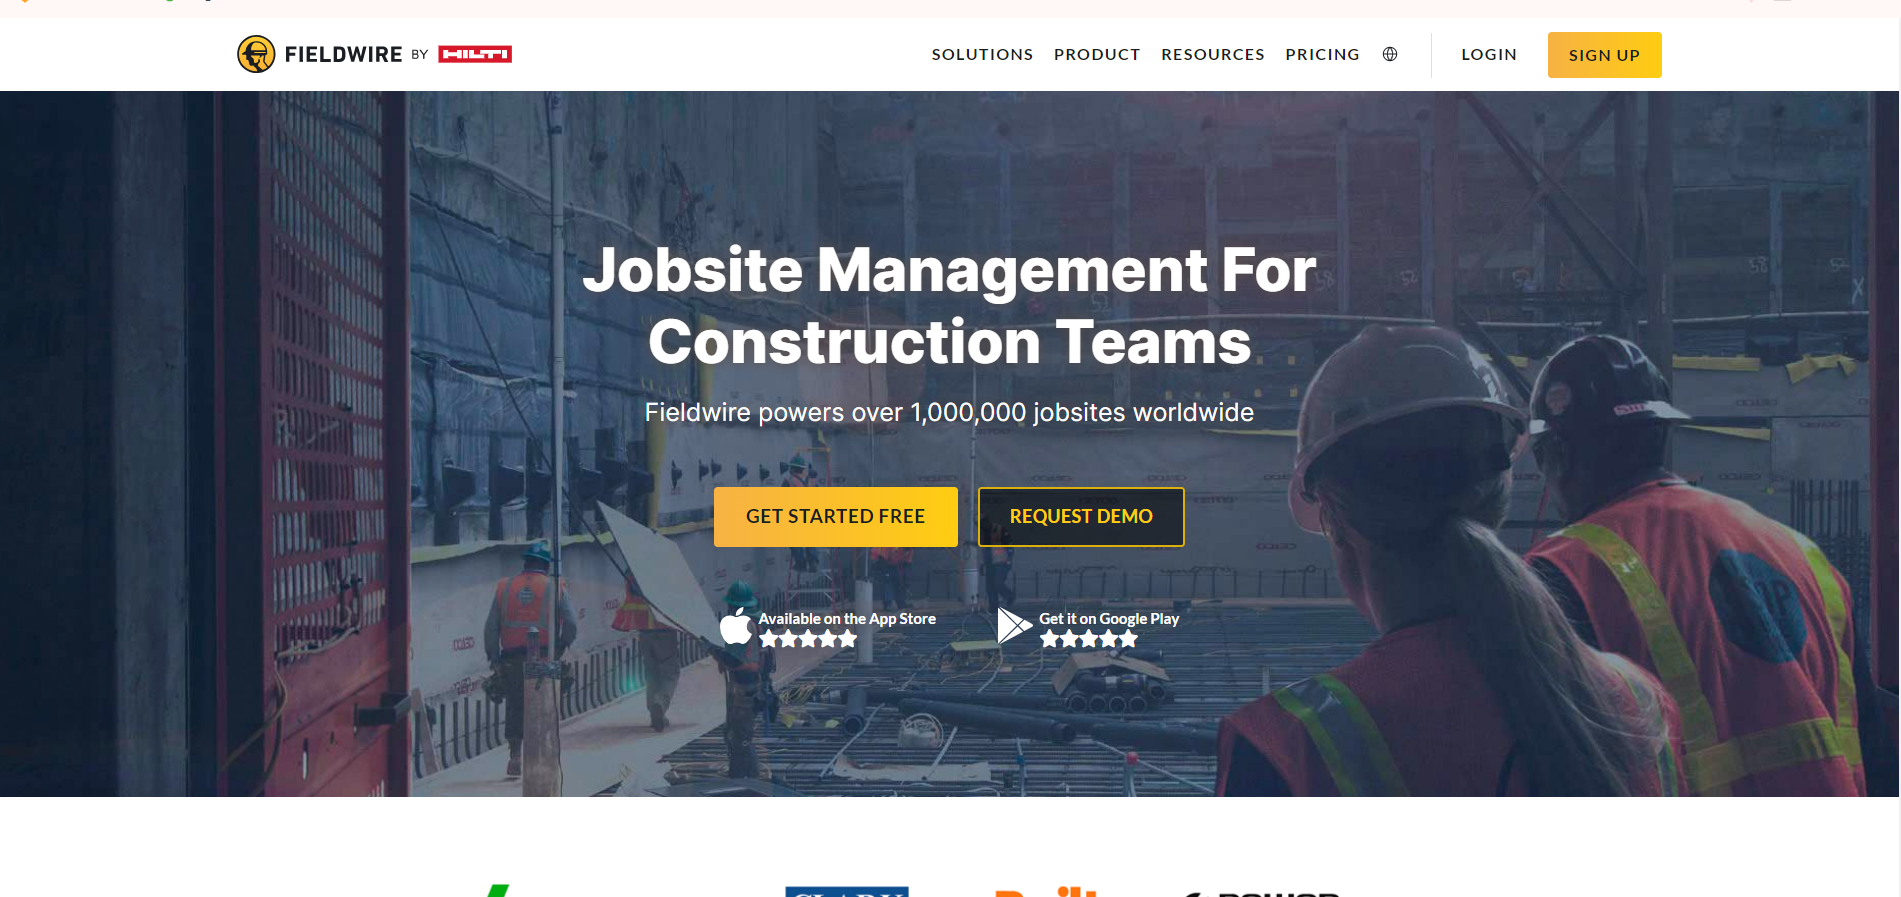
\includegraphics[width=\linewidth]{src/assets/chapters/fieldwire.PNG}
    \caption{Fieldwire Homepage}
    \label{fig:fieldwire_image}
\end{figure}

\subsection{MyHammer}
MyHammer is an online platform based in Germany that connects homeowners and businesses with local tradesmen and service providers for various construction, renovation, and repair projects. MyHammer provides various features including a wide range of services, a transparent bidding process, a mobile-friendly interface

\begin{figure}[H]
    \centering
    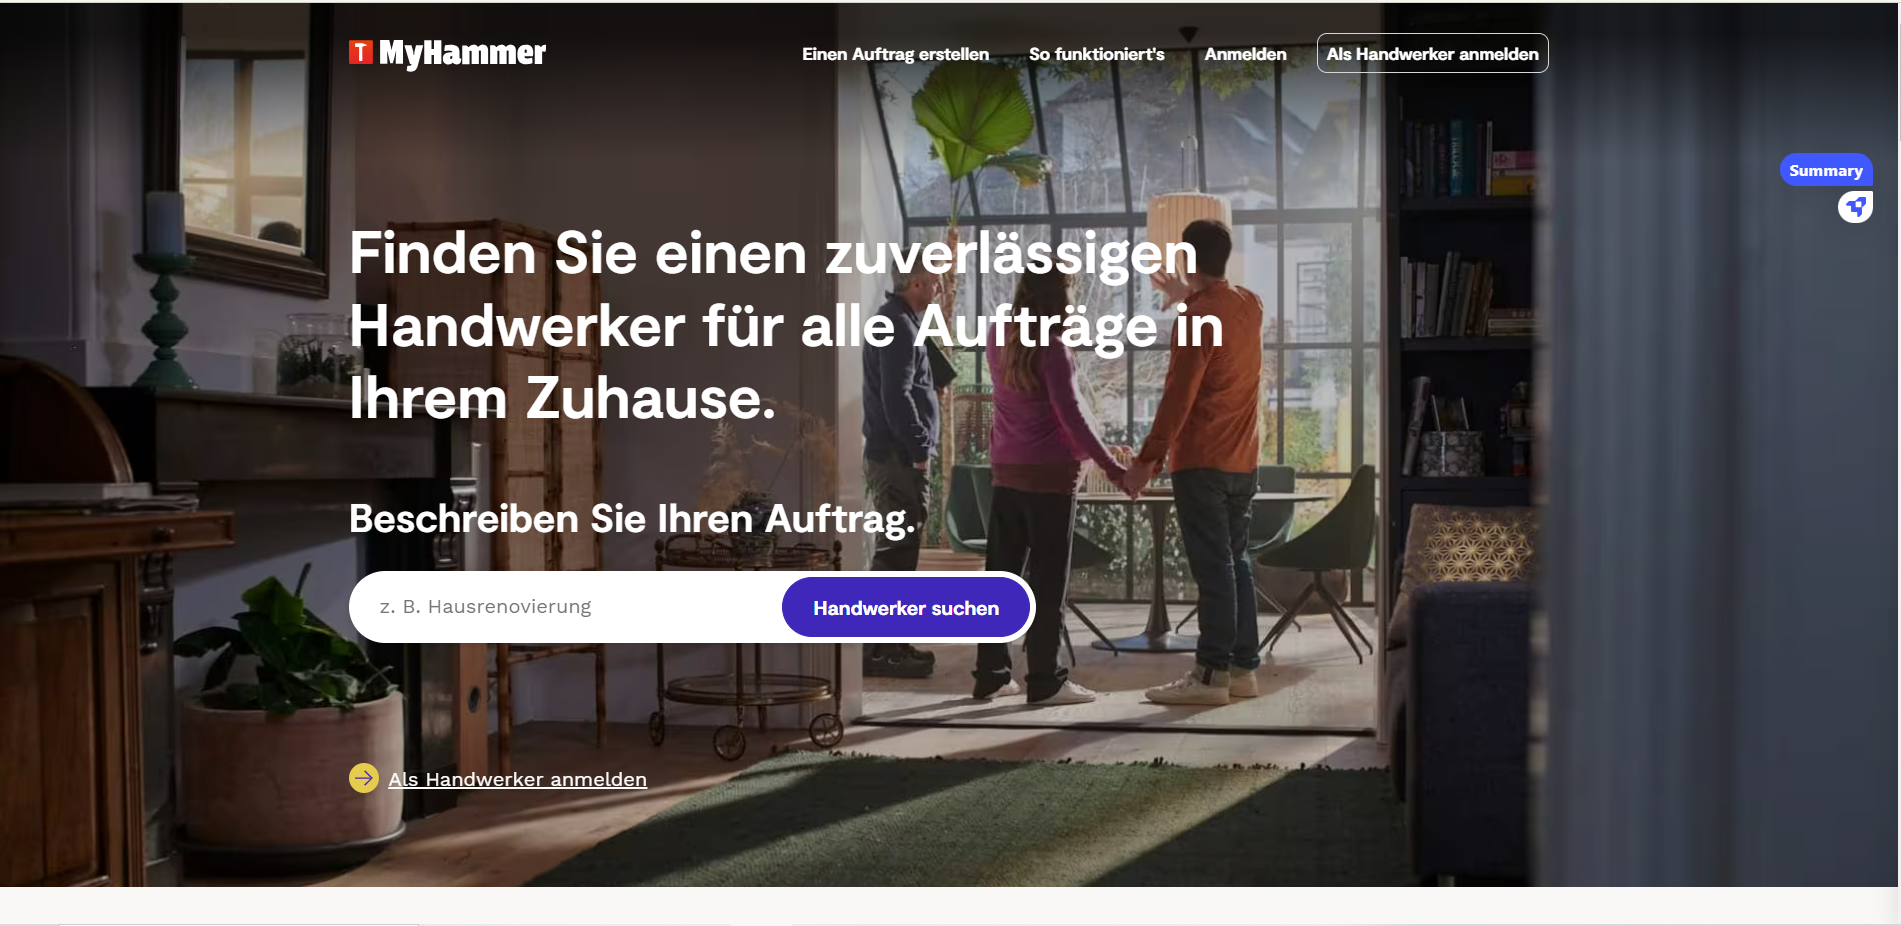
\includegraphics[width=\linewidth]{src/assets/chapters/myHammer.PNG}
    \caption{MyHammer Homepage}
    \label{fig:myhammer_image}
\end{figure}

\subsection{Competitors Selection}
We're conducting a thorough assessment of project management platforms for industrial climbers to improve user experience and streamline operational processes. By evaluating their functionalities, strengths, and weaknesses against 7 (maybe more) key criteria tailored to our project's needs, we aim to select the platform that best meets our requirements.

\begin{itemize}
    \item \textbf{C1: User Interface:} The platform's interface design, including ease of navigation and overall user experience for technicians and project managers.
    \item \textbf{C2: Task Management:} The platform's capability to efficiently manage tasks related to industrial climbing projects, including task assignment, progress tracking, and deadline setting.
    \item \textbf{C3: Document Management:} Features for organizing and managing project documents such as permits, safety procedures, and equipment manuals relevant to industrial climbing projects.
    \item \textbf{C4: Communication Tools:} The platform's communication features, including real-time messaging, notifications, and collaboration tools facilitate effective communication among team members.
    \item \textbf{C5: Safety Compliance:} The platform's ability to ensure compliance with safety regulations and standards pertinent to industrial climbing projects, such as tracking certifications, training records, and safety procedures.
    \item \textbf{C6: Equipment Management:} Tools for managing equipment used in industrial climbing projects, including tracking inspections, certifications, and maintenance records to ensure safety and compliance.
    \item \textbf{C7: Project Planning and Scheduling:} Features for project planning and scheduling, including resource allocation, timeline management, and task dependencies, relevant to industrial climbing projects.
\end{itemize}

\begin{longtable}{|p{2cm}|p{2.5cm}|p{2.5cm}|p{2.5cm}|p{2.5cm}|}
    % Table header information for the first part
    \caption{Comparison of Project Management Platforms for Industrial Climbers} \\
    \hline
    \textbf{Criteria} & \textbf{MyHammer} & \textbf{Blauarbeit} & \textbf{Fieldwire} & \textbf{IRATA Hub} \\
    \hline
    \endfirsthead
    
    % Table continuation header information
    \hline
    \textbf{Criteria} & \textbf{MyHammer} & \textbf{Blauarbeit} & \textbf{Fieldwire} & \textbf{IRATA Hub} \\
    \hline
    \endhead
    
    % Footer at the end of each page (if needed)
    \hline
     
    
    % Footer at the end of the table (if needed)
    \hline
    \endlastfoot
    
    % Table content for Part 1
    C1: User Interface &  User-friendly interface for homeowners and service providers to connect for home improvement projects. & Straightforward interface for customers and service providers to post and bid on household service tasks. & Modern interface designed for construction teams, offering plan viewing and task management on desktop and mobile. & Professional interface for industrial rope access professionals, providing resources and job listings in an organized format. \\ 
    \hline
    C2: Task Management & MyHammer lacks dedicated task management features for organizing and tracking project progress. & Blauarbeit also lacks dedicated task management features. While it facilitates the posting and bidding on tasks related to household services, it does not offer tools specifically for task management within projects. & Fieldwire excels in task management for construction projects, offering robust features such as assigning tasks, tracking progress, attaching documents, and communicating with team members, all within a centralized platform. & IRATA Hub is not primarily focused on task management. While it provides resources and job listings for industrial rope access professionals, it does not offer dedicated task management tools for organizing work within projects. \\
    \hline
    C3: Document Management & No dedicated document management features for home improvement projects. & Does not offer specific tools for document management. & Excellent document management for construction projects, including uploading, annotating, and tracking revisions. & No focus on document management; primarily serves as a resource hub for industrial rope access professionals. \\
    \hline
    
    % Table content for Part 2, continues in the same longtable environment
    C4: Communication Tools & Offers basic communication tools for homeowners and service providers to discuss project details and negotiate terms within the platform. & Provides standard communication channels for customers and service providers to communicate regarding job requirements and arrangements. & Includes robust communication features tailored for construction teams, allowing for real-time collaboration, messaging, and file sharing among team members within projects. & IRATA Hub does not offer specific communication tools within the platform. \\
    \hline
    C5: Safety Compliance & No specific safety compliance features for home improvement projects. & No dedicated safety compliance features for household services. & Robust safety compliance tools for construction projects, including checklists and real-time updates. & IRATA Hub provides resources for safety practices but lacks specific safety compliance features. \\
    \hline
    C6: Equipment Management & MyHammer's equipment management system is integrated, offering automated tracking and management of equipment assets for efficient project execution. & Blauarbeit's equipment management feature is automated, providing scalable solutions for tracking and managing equipment assets across projects. & Fieldwire's equipment management system is scalable, offering seamless integration with project workflows and efficient management of equipment assets. & IRATA Hub's equipment management feature enables precise tracking and management of equipment assets, ensuring optimal utilization and maintenance. \\
    \hline
    C7: Project Planning and Scheduling & No specific project planning or scheduling tools provided. & Lacks dedicated project planning and scheduling features. & Offers comprehensive project planning and scheduling tools for construction projects, including Gantt charts and task dependencies. & Does not focus on project planning and scheduling within the platform. \\
    \hline
\end{longtable}

% ----------------------- Assessment of the case ----------------------- %
\section{Assessment of the case}
\subsection{Describing the work procedure}
The work on any project must first of all be preceded by a thorough study of the existing ones which undermines the strengths and weaknesses of the current system, as well as the business decisions that should be taken into account during the conception as well as the realization.

\subsection{Criticizing the current state}
After studying the existing, we can determine its limitations:

\subsubsection{Functional Issues}
\begin{itemize}
    \item Functionalities are not working as expected.
    \item New features are still not developed.
    \item Parts of the application need complete changes to satisfy the client's requirements.
\end{itemize}

\subsubsection{Technical Issues}
\begin{itemize}
    \item Since cron jobs are running for the whole day, bugs are hard to respond to fast enough because we can only deploy once at the end of the day.
    \item Many bugs remain unfixed.
    \item The code needs refactoring due to some bad practices that make the app take more time to execute.
\end{itemize}

\subsection{Proposed solution}
To address the identified issues, we propose the following solutions. First, we will focus on enhancing existing features to ensure they work as expected. This includes a thorough review and testing of the functionalities to identify and fix any bugs. Additionally, we will prioritize the development of new features to meet the client's requirements. Comprehensive refactoring of the codebase will be undertaken to eliminate bad practices and improve performance. We also suggest improving the UI/UX design to enhance user experience and satisfaction. By implementing these solutions, we aim to significantly improve the application's overall performance, reliability, and user satisfaction.

\subsection{Work to Be Done}
\begin{itemize}
    \item Develop the major feature: the reward system.
    \item  Deploy the reward system into staging and then production.
    \item Enhance existing features to ensure they work as expected.
    \item Conduct a thorough review and testing of functionalities to identify and fix any bugs.
    \item Develop new features to meet the client's requirements.
    \item Refactor the codebase to eliminate bad practices and improve performance.
    \item Improve the UI/UX design to enhance user experience and satisfaction.
\end{itemize}
x
% ----------------------- Development Methodology ----------------------- %
\section{Development Methodology}
\subsection{Agile methodology}
Agile is a structured and iterative approach to project management and product development.
It recognizes the volatility of product development, and provides a methodology for self-organizing teams to respond to change without going off the rails.

\subsection{Scrum methodology}
Scrum teams commit to completing an increment of work, which is potentially shippable, through set intervals called sprints.
Their goal is to create learning loops to quickly gather and integrate customer feedback.
Scrum teams adopt specific roles, create special artifacts, and hold regular ceremonies to keep things moving forward.


\begin{figure}[H]
    \centering
    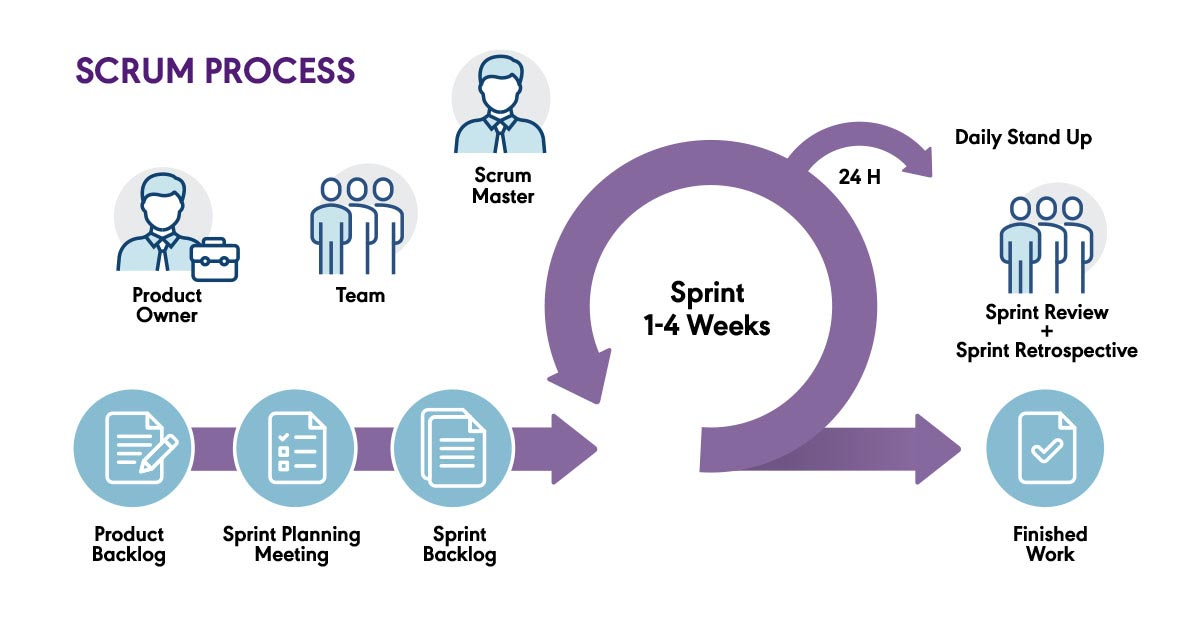
\includegraphics[width=0.7\textwidth]{src/assets/chapters/blog-scrum-process-opt.jpg}
    \caption{The Scrum Framework}
    \label{fig:Scrum_Framework_image}
\end{figure}


\subsection{Kanban methodology}
Kanban is all about visualizing your work, limiting work in progress, and maximizing efficiency (or flow).
Kanban teams focus on reducing the time a project takes from start by using a Kanban board to continuously improve their flow of work.
To explain more in details, Kanban is based on a continuous workflow structure that keeps teams nimble and ready to adapt to changing priorities.
Work items —represented by cards— are organized on the board where they flow from one stage of the workflow or column to the next.
Common workflow stages are To Do, In Progress, In Review, and Done.

\subsection{Scrumban methodology}
Scrumban is a hybrid Agile methodology that combines elements of Scrum and Kanban. Here are key points about Scrumban:

\begin{itemize}
    \item Hybrid Methodology: Scrumban blends the flexibility of Kanban with the structure of Scrum to optimize workflow.
    \item Continuous Improvement: Like Kanban, Scrumban emphasizes continuous improvement through visualizing workflow and limiting Work in Progress (WIP).
    \item Iterative Approach: Scrumban maintains Scrum's iterative approach, allowing for regular review and adaptation of processes.
    \item Adaptive Planning: Scrumban enables adaptive planning, allowing teams to adjust priorities and resources based on changing requirements.
    \item Lean Principles: Scrumban incorporates Lean principles, such as eliminating waste and maximizing value delivery, to streamline processes.
\end{itemize}

\begin{figure}[H]
    \centering
    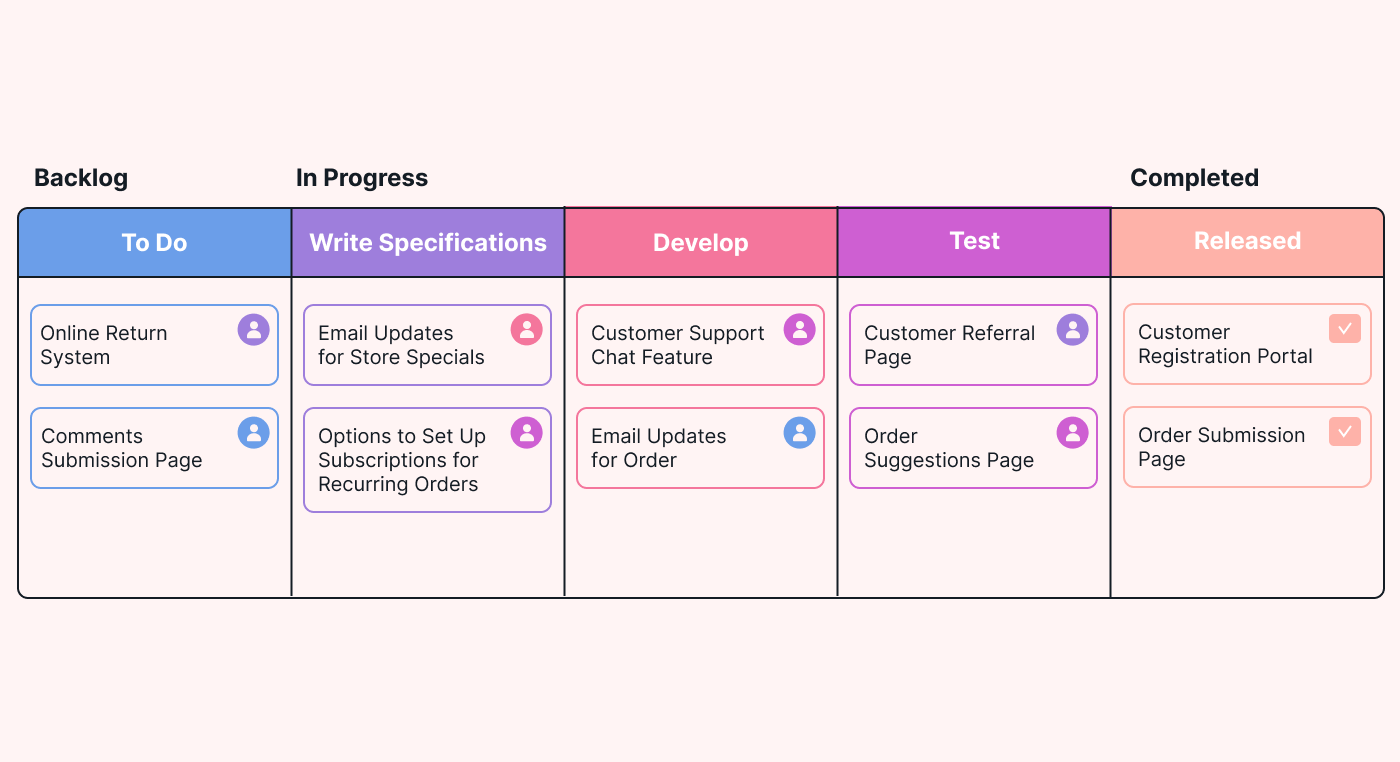
\includegraphics[width=0.7\textwidth]{src/assets/chapters/Scrumban.png}
    \caption{The Scrumban board}
    \label{fig:Scrumban_image}
\end{figure}

\subsection{The choice for AERMAX}
Scrumban has been chosen as the preferred development methodology for the following reasons:
\begin{itemize}
    \item \textbf{Flexibility:} Flexibility is a key characteristic of Scrumban, as it combines the structure of Scrum with the adaptability of Kanban. This allows teams to respond quickly to changes in priorities or requirements, while still having a framework to guide their work.
    \item \textbf{Continuous Improvement:} Continuous improvement is strongly encouraged in Scrumban, as teams are allowed to evolve their processes over time. Regular reflection and adjustment promote more efficient workflows, leading to a more productive development process.
    \item \textbf{Reduced Waste:} Scrumban helps reduce waste in the development process by emphasizing just-in-time delivery and limiting work in progress. Teams focus on completing tasks before starting new ones, which leads to a smoother flow and faster delivery.
    \item \textbf{Improved Visibility:} With Scrumban's visual boards, teams have improved visibility into their work. Everyone can see what tasks are in progress, what's completed, and what's next, fostering transparency and collaboration.
    \item \textbf{Optimized Flow:} Scrumban optimizes flow by balancing the flexibility of Kanban with the structured approach of Scrum. This enables teams to deliver value more consistently and predictably, leading to happier customers and stakeholders.
\end{itemize}

\begin{figure}[H]
    \centering
    \makebox[\textwidth]{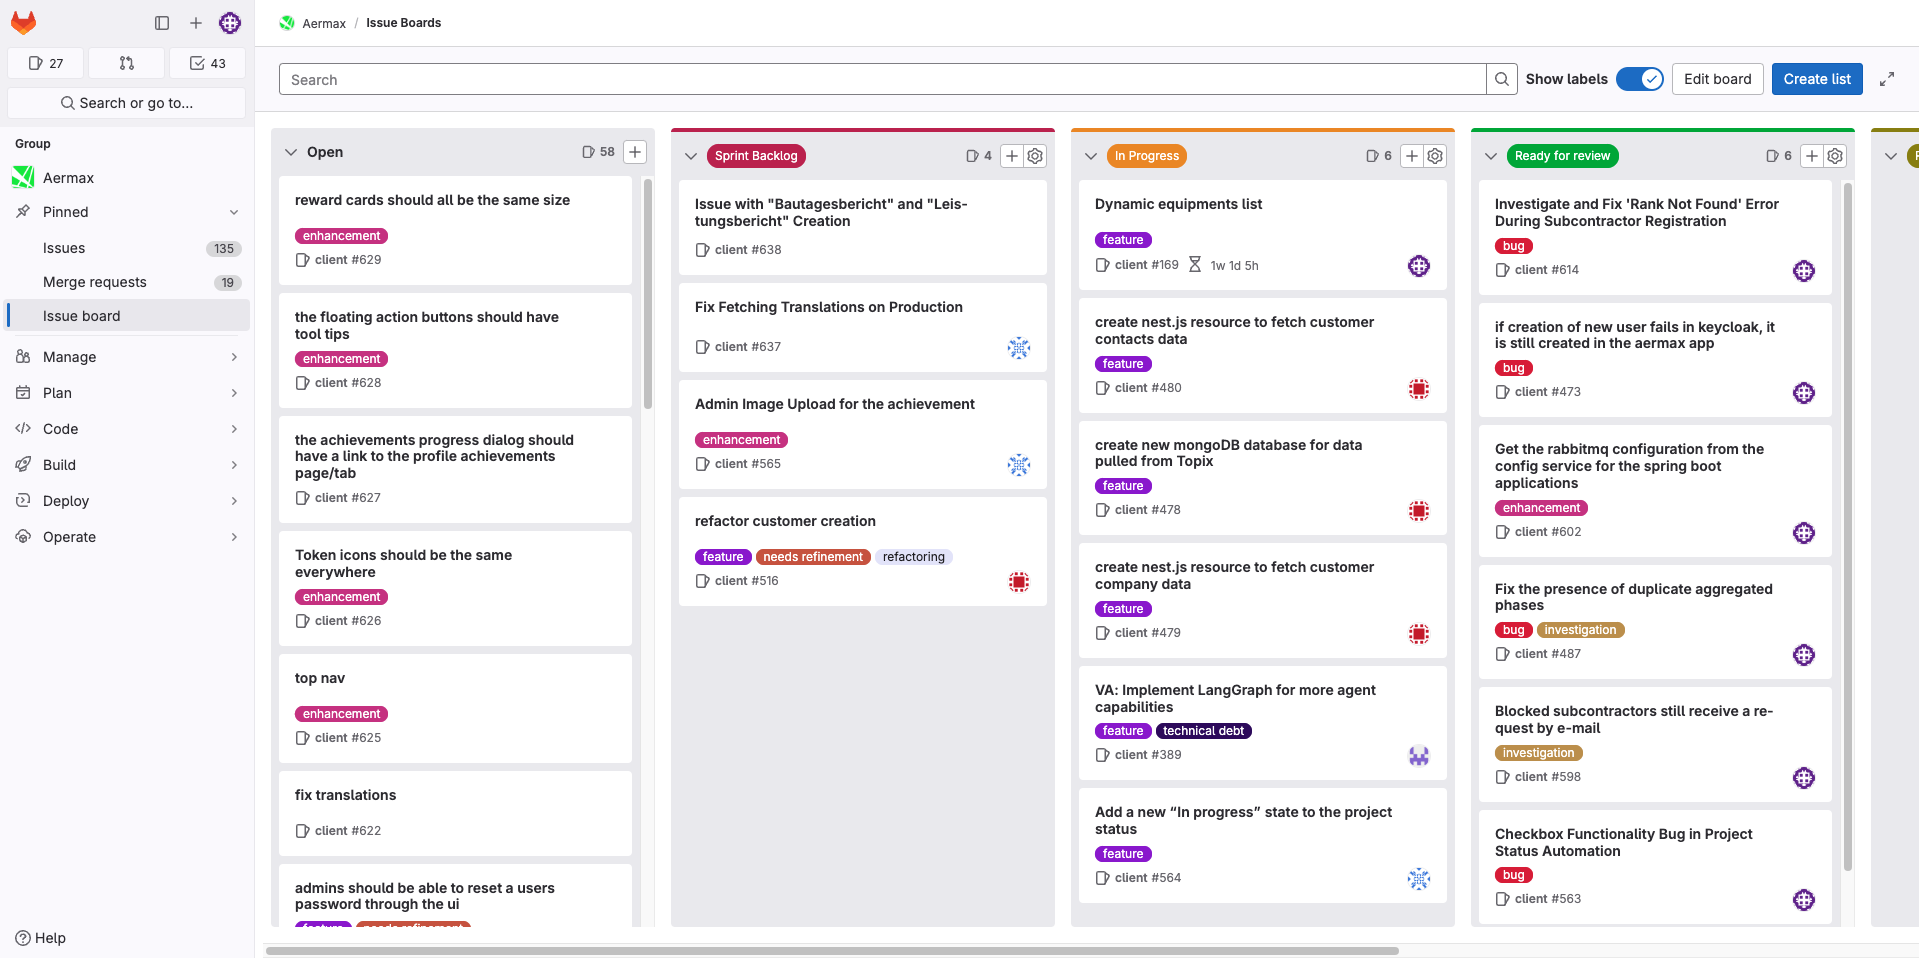
\includegraphics[width=14cm]{src/assets/chapters/aermax-board.png}}
    \caption{Aermax Board}
    \label{fig:armax-board}
\end{figure}
 
\subsection{Unified Modeling Language}
The Unified Modeling Language (UML) is a general-purpose, developmental, modeling language in the field of software engineering that is intended to provide a standard way to visualize the design of a system. In our case, we used UML to design the top level view of the systems therefore we only used the Use Case and Sequence diagrams.

\section{General Team Structure}
The Aermax project team is composed of diverse and skilled professionals, each bringing unique expertise to the project. Below is the general team structure:

\begin{itemize}
    \item \textbf{Anis Benna} is the lead developer, responsible for overseeing the development process and ensuring the technical direction aligns with the project's goals.
    \item \textbf{Robert Könitz} acts as a mentor and sparring partner, providing guidance, support, and valuable insights to the development team.
    \item \textbf{Joachim Liedtke} an experienced developer, contributing significantly to the project's advancement with his extensive knowledge and skills.
    \item \textbf{Donia Skima \& Ramez Taher} we joined as interns, bringing fresh perspectives and assisting with various development tasks while gaining valuable hands-on experience.
\end{itemize}

This collaborative team structure ensures that the project benefits from a blend of leadership, mentorship, experienced development, and innovative ideas from interns, fostering a dynamic and productive working environment.


\setcounter{secnumdepth}{0} % Set the section counter to 0 so next section is not counted in toc
% ----------------------- Conclusion ----------------------- %
\section{Conclusion}
In conclusion, this chapter began with an introduction to the host organization, followed by a detailed assessment of the identified problems and their associated challenges. We then proceeded to evaluate the competitive landscape to understand the key issues we aim to address. Lastly, we described our team’s adoption of an agile methodology, emphasizing its role in enhancing flexibility and collaboration. The upcoming chapter will delve into Sprint 0, marking the commencement of the project. This phase involves establishing objectives and laying out the roadmap for subsequent sprints.
